%%%%%%%%%%%%%%%%%%%%%%%%%%%%%%%%%%%%%%%%%
% Beamer Presentation
% LaTeX Template
% Version 1.0 (10/11/12)
%
% This template has been downloaded from:
% http://www.LaTeXTemplates.com
%
% License:
% CC BY-NC-SA 3.0 (http://creativecommons.org/licenses/by-nc-sa/3.0/)
%
%%%%%%%%%%%%%%%%%%%%%%%%%%%%%%%%%%%%%%%%%

%----------------------------------------------------------------------------------------
%	PACKAGES AND THEMES
%----------------------------------------------------------------------------------------

\documentclass{beamer}

\mode<presentation> {

% The Beamer class comes with a number of default slide themes
% which change the colors and layouts of slides. Below this is a list
% of all the themes, uncomment each in turn to see what they look like.

%\usetheme{default}
%\usetheme{AnnArbor}
%\usetheme{Antibes}
%\usetheme{Bergen}
%\usetheme{Berkeley}
%\usetheme{Berlin}
%\usetheme{Boadilla}
%\usetheme{CambridgeUS}
%\usetheme{Copenhagen}
%\usetheme{Darmstadt}
%\usetheme{Dresden}
\usetheme{Frankfurt}
%\usetheme{Goettingen}
%\usetheme{Hannover}
%\usetheme{Ilmenau}
%\usetheme{JuanLesPins}
%\usetheme{Luebeck}
%\usetheme{Madrid}
%\usetheme{Malmoe}
%\usetheme{Marburg}
%\usetheme{Montpellier}
%\usetheme{PaloAlto}
%\usetheme{Pittsburgh}
%\usetheme{Rochester}
%\usetheme{Singapore}
%\usetheme{Szeged}
%\usetheme{Warsaw}


% As well as themes, the Beamer class has a number of color themes
% for any slide theme. Uncomment each of these in turn to see how it
% changes the colors of your current slide theme.

%\usecolortheme{albatross}
%\usecolortheme{beaver}
%\usecolortheme{beetle}
%\usecolortheme{crane}
%\usecolortheme{dolphin}
%\usecolortheme{dove}
%\usecolortheme{fly}
%\usecolortheme{lily}
%\usecolortheme{orchid}
%\usecolortheme{rose}
%\usecolortheme{seagull}
%\usecolortheme{seahorse}
%\usecolortheme{whale}
%\usecolortheme{wolverine}

%\setbeamertemplate{footline} % To remove the footer line in all slides uncomment this line
%\setbeamertemplate{footline}[page number] % To replace the footer line in all slides with a simple slide count uncomment this line

%\setbeamertemplate{navigation symbols}{} % To remove the navigation symbols from the bottom of all slides uncomment this line
}

\usepackage{graphicx} % Allows including images
\usepackage{booktabs} % Allows the use of \toprule, \midrule and \bottomrule in tables
\usepackage{amsmath}
\usepackage{xcolor}
\usepackage{graphicx}
\usepackage{ragged2e}
% \usepackage{natbib} 
%\usepackage[style=authoryear,maxcitenames=1,maxnames = 50]{biblatex}
% \usepackage{biblatex}
\usepackage{forest}
\usepackage{tikz}
\usetikzlibrary{shapes,arrows,positioning,automata}
\usepackage{changepage}
\usepackage{xcolor}
\usepackage{subcaption}

% \usepackage[demo]{graphicx}

% Beamer theme font
\usefonttheme{structurebold} % bold titles

% \renewcommand*{\nameyeardelim}{\addcomma\addspace}

% \addbibresource{wileyNJD-APA.bib}

\setbeamertemplate{bibliography item}[text]

% \setbeamersize{text margin left=3mm,text margin right=3mm} 

%----------------------------------------------------------------------------------------
%	TITLE PAGE
%----------------------------------------------------------------------------------------

\title[]{Joint Mixture of Hidden Markov Models for Actigraphy Data} % The short title appears at the bottom of every slide, the full title is only on the title page

% \author{Jordan Aron, Paul Albert, and Mark Fiecas} % Your name
\institute[] % Your institution as it will appear on the bottom of every slide, may be shorthand to save space
{
\\ % Your institution for the title page
%\medskip
%\textit{john@smith.com} % Your email address
}
% \date{December 13, 2024} % Date, can be changed to a custom date

\begin{document}



\begin{frame}
\titlepage % Print the title page as the first slide
\end{frame}



%----------------------------------------------------------------------------------------
%	PRESENTATION SLIDES
%----------------------------------------------------------------------------------------

%------------------------------------------------

\section{Introduction} 
%------------------------------------------------
\begin{frame}
\frametitle{Motivation}
\begin{itemize}

    \item The sleep/wake cycle plays a major role in health
    \item Reduced physical activity is associated with increased all-cause mortality
    \item Goal: connect the sleep/wake cycle and activity to mortality risk
    

\end{itemize}

\end{frame}

%------------------------------------------------
\begin{frame}
\frametitle{Motivating Example}
\begin{itemize}
    \item The National Health and Nutrition Examination Survey (NHANES) is a national examination survey dating back to the 1960s
    \item Designed to assess the health and nutrition of the U.S. using a combination of physical examinations, lab tests, and interviews

\end{itemize}

\end{frame}
%------------------------------------------------

\begin{frame}{Actigraphy}
\begin{itemize}
    \item Actigraphy data from 2011-2012 and 2013-2014
    \item Directly measure activity and light
    \item Infer sleep/wake cycle using observed measurements
    \item Light helps with determining sedentary behavior
\end{itemize}
\end{frame}
%------------------------------------------------
\begin{frame}
\frametitle{Motivation}
\begin{itemize}

    \item Approach: use physical activity monitors (PAMs) to examine activity and light and then infer the sleep/wake cycle
    \item Sleep studies are expensive and often limited in size
    \item Self reported sleep and activity metrics are often unreliable 
    \item PAMs are not without their own quirks
    % https://pmc.ncbi.nlm.nih.gov/articles/PMC3798642/#:~:text=This%20study%20found%20that%20self,and%20wake%20after%20sleep%20onset.

\end{itemize}

\end{frame}


%%------------------------------------------------
\begin{frame}
\frametitle{Data Description}
\begin{itemize}
    \item Longitudinal activity and light data
    \item Time-to-event linked mortality data
    %Data is one measurement per minute for a week per person
\end{itemize}
\includegraphics[scale = .2]{SampleActivity.jpg}

\end{frame}


\section{Model Description} 

\begin{frame}{Joint Latent Class Model}
\begin{itemize}
    \item Assumes latent class structure entirely captures the relationship between longitudinal and survival data
    \item Mixture of hidden Markov models (MHMM) for the longitudinal component
    \item Cox model for the survival aspect
    \item Joint model can incorporate uncertainty in latent class prediction
\end{itemize}
\end{frame}

%------------------------------------------------



\begin{frame}
\frametitle{Markov Model}

\begin{center}
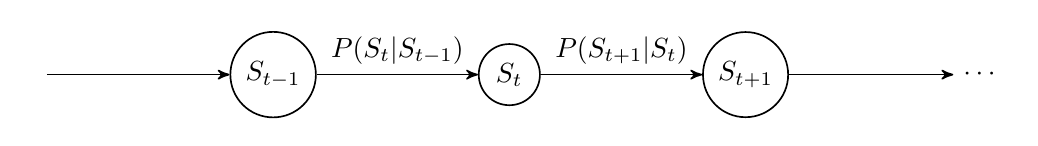
\begin{tikzpicture}[->, >=stealth', auto, semithick, node distance=3cm]

\tikzstyle{every state}=[
    fill=white,
    draw=black,
    thick,
    text=black,
    scale=0.9
]

\node[circle, draw] (S_0) {$S_{t-1}$};
\node[circle, draw] (S_1) [right of=S_0] {$S_t$};
\node[circle, draw] (S_2) [right of=S_1] {$S_{t+1}$};
\node[] (Dot) [right of=S_2] {$\cdots$};
\node[] (Hid) [left of=S_0] {};

\path
(S_0) edge node {$P(S_t|S_{t-1})$} (S_1)
(S_1) edge node {$P(S_{t+1}|S_t)$} (S_2)
(S_2) edge (Dot)
(Hid) edge node {} (S_0);

\end{tikzpicture}
\end{center}

\end{frame}

%------------------------------------------------

\begin{frame}
\frametitle{Hidden Markov Model}

\begin{center}
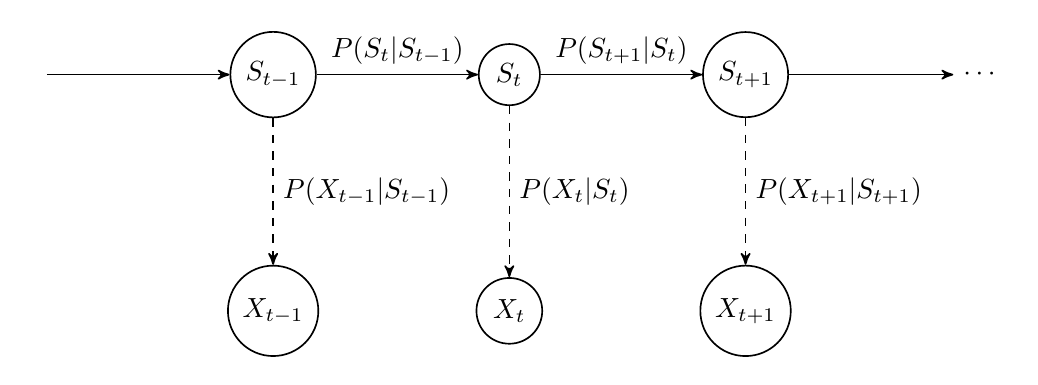
\begin{tikzpicture}[->, >=stealth', auto, semithick, node distance=3cm]

\tikzstyle{every state}=[
    fill=white,
    draw=black,
    thick,
    text=black,
    scale=0.9
]

\node[circle, draw] (S_0) {$S_{t-1}$};
\node[circle, draw] (S_1) [right of=S_0] {$S_t$};
\node[circle, draw] (S_2) [right of=S_1] {$S_{t+1}$};
\node[] (Dot) [right of=S_2] {$\cdots$};
\node[] (Hid) [left of=S_0] {};

\node[circle, draw] (X_0) [below of=S_0] {$X_{t-1}$};
\node[circle, draw] (X_1) [below of=S_1] {$X_t$};
\node[circle, draw] (X_2) [below of=S_2] {$X_{t+1}$};

\path
(S_0) edge node {$P(S_t|S_{t-1})$} (S_1)
(S_1) edge node {$P(S_{t+1}|S_t)$} (S_2)
(S_2) edge (Dot)
(Hid) edge node {} (S_0)
(S_0) edge[dashed] node {$P(X_{t-1}|S_{t-1})$} (X_0)
(S_1) edge[dashed] node {$P(X_t|S_t)$} (X_1)
(S_2) edge[dashed] node {$P(X_{t+1}|S_{t+1})$} (X_2);

\end{tikzpicture}
\end{center}

\end{frame}




\begin{frame}
\frametitle{Bivariate Hidden Markov Model}
\begin{center}
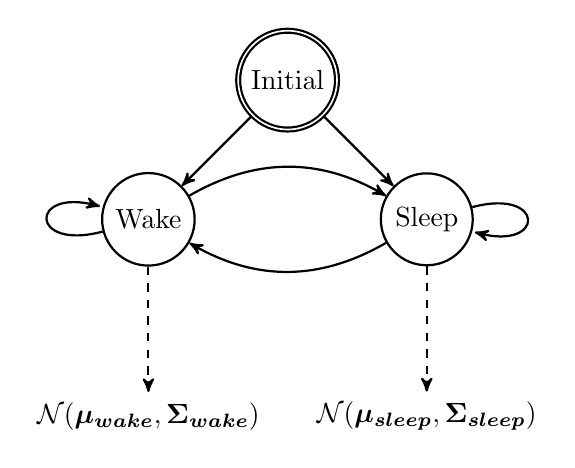
\begin{tikzpicture}[->, >=stealth', thick, node distance=2.5cm]

\tikzstyle{every state}=[fill=white,draw=black,thick,text=black,scale=.5]

\node[circle,draw,double] (Init)            {Initial};
\node[circle, draw] (Wake)[below left of=Init] {Wake}; 
\node[circle, draw] (Sleep)[below right of=Init] {Sleep}; 
\node[] (EmitW)[below of=Wake] {$\mathcal{N}(\boldsymbol{\mu_{wake}},\boldsymbol{\Sigma_{wake}})$};
\node[] (EmitS)[below of=Sleep] {$\mathcal{N}(\boldsymbol{\mu_{sleep}},\boldsymbol{\Sigma_{sleep}})$};
%\node[circle, draw] (S0B)[below below of =S_0] {$S_1$}


\path
(Init) edge (Wake)
(Init) edge (Sleep)
(Sleep) edge[loop right] (Sleep)
(Wake) edge[loop left] (Wake)
(Sleep) edge[bend left] (Wake)
(Wake) edge[bend left] (Sleep)

(Wake) edge[dashed] (EmitW)
(Sleep) edge[dashed] (EmitS);
\end{tikzpicture}
\end{center}
\end{frame}

%------------------------------------------------


\begin{frame}
\frametitle{Example}
\begin{itemize}
    \item Subgroup A: wakes up early, active, and tend to live longer
    \item Subgroup B: sleeps in, sedentary, and die earlier
    \item Estimate MHMM and survival parameters jointly 
    %compare to two-stage
\end{itemize}
\end{frame}

% A Markov chain is a stochastic model describing a sequence of possible events in which the probability of each event depends only on the state attained in the previous event


\begin{frame}
\frametitle{Mixture of Bivariate Hidden Markov Models}
\begin{center}
\begin{tikzpicture}[->, >=stealth', thick, node distance=2.5cm,transform canvas={scale=.8}]

\tikzstyle{every state}=[fill=white,draw=black,thick,text=black,scale=.5]

\node[](Init) {};
\node[] (InitL)[above left of=Init] {};
\node[] (InitR)[above right of=Init] {};
\node[draw, double] (InitReal)[above right of=InitL] {Start};

\node[circle,draw,double,red] (Init1)[below left of=InitL]     {Initial A};
\node[] (GA)[above of=Init1,red] {If member of group A};
\node[circle, draw,red] (Wake1)[below left of=Init1] {Wake}; 
\node[circle, draw,red] (Sleep1)[below right of=Init1] {Sleep}; 
\node[red] (EmitW1)[below of=Wake1] {$\mathcal{N}(\boldsymbol{\mu_{wake}^{(A)}},\boldsymbol{\Sigma_{wake}^{(A)}})$};
\node[red] (EmitS1)[below of=Sleep1] {$\mathcal{N}(\boldsymbol{\mu_{sleep}^{(A)}},\boldsymbol{\Sigma_{sleep}^{(A)}})$};

\node[circle,draw,double,blue] (Init2)[below right of=InitR]     {Initial B};
\node[] (GB)[above of=Init2,blue] {If member of group B};
\node[circle, draw,blue] (Wake2)[below left of=Init2] {Wake}; 
\node[circle, draw,blue] (Sleep2)[below right of=Init2] {Sleep}; 
\node[blue] (EmitW2)[below of=Wake2] {$\mathcal{N}(\boldsymbol{\mu_{wake}^{(B)}},\boldsymbol{\Sigma_{wake}^{(B)}})$};
\node[blue] (EmitS2)[below of=Sleep2] {$\mathcal{N}(\boldsymbol{\mu_{sleep}^{(B)}},\boldsymbol{\Sigma_{sleep}^{(B)}})$};


\path
(InitReal) edge[red] (Init1)
(InitReal) edge[blue] (Init2)

(Init1) edge[red] (Wake1)
(Init1) edge[red] (Sleep1)
(Sleep1) edge[red,loop right] (Sleep1)
(Wake1) edge[red,loop left] (Wake1)
(Sleep1) edge[red,bend left] (Wake1)
(Wake1) edge[red,bend left] (Sleep1)

(Init2) edge[blue] (Wake2)
(Init2) edge[blue] (Sleep2)
(Sleep2) edge[loop right,blue] (Sleep2)
(Wake2) edge[loop left,blue] (Wake2)
(Sleep2) edge[bend left,blue] (Wake2)
(Wake2) edge[bend left,blue] (Sleep2)

(Wake1) edge[red,dashed] (EmitW1)
(Sleep1) edge[red,dashed] (EmitS1)

(Wake2) edge[blue,dashed] (EmitW2)
(Sleep2) edge[blue,dashed] (EmitS2);
\end{tikzpicture}
\end{center}
\end{frame}

% \begin{frame}{Notation}
% \begin{itemize}
%     \item  $\textbf{S} = \{S_{1}, S_{2}, ..., S_{T}\}$ is the first  order Markov chain of latent states and is fully described by $P(S_{1})$ and $P(S_{t}|S_{t-1})$
%     \item $\textbf{a} = \{a_{1}, a_{2}, ..., a_{T}\}$ is the vector of observed activity values
%     \item $\textbf{l} = \{l_{1}, l_{2}, ..., l_{T}\}$ is the vector of observed light values
    
%     \item Conditional independence: $P(a_{t}, l_t|\textbf{S}) = P(a_{t}, l_t|S_{t})$
% \end{itemize}
% \end{frame}

\begin{frame}{HMM Parameters}
\begin{itemize}
    \item HMM assignment determined by latent class membership
    \item Harmonic transition matrix
    \item NHANES sample weights
    \item Bivariate Normal emission distribution
\end{itemize}
\end{frame}



\begin{frame}{Limit of Detection (LoD)}
\begin{itemize}
    \item Light values are often below the limit of detection
    \item Tobit approach, replace PDF with CDF when below LoD
\end{itemize}
\end{frame}

\begin{frame}{Survival Model}
\begin{itemize}
    \item Cox model accounting for latent class and age
    \item Breslow estimator for non-parametric baseline hazards
    %\item P(group A | data) = $\frac{\text{P(data | group A)P(group A)}}{\text{P(data)}}$
\end{itemize}
\end{frame}
%------------------------------------------------

 \begin{frame}{Model Diagram}
 \begin{figure}
     \centering
     \includegraphics[width=0.95\linewidth]{ModelDiagram.pdf}
    %  \caption{Survival coefficient confidence interval coverage by model type and mixture for 250 simulations with 3,000 individuals each.}
    %  \label{fig:enter-label}
 \end{figure}
 \end{frame}

\section{Estimation} 


\begin{frame}{EM Algorithm}
\begin{itemize}
    \item Write likelihood as if latent variables are known using indicator functions
    \item Replace log likelihood with the expectation of the log likelihood conditional on the observed data
\end{itemize}
\end{frame}
%------------------------------------------------

\begin{frame}{Notation}
\begin{itemize}
    \item Let \textbf{a} and \textbf{x} be the observed activity and light data
    \item Let t be the observed survival time and $\delta$ be the censored indicator
    \item Let \textbf{S} be the latent sleep/wake state
    \item Let \textbf{G} be the latent subgroup assignment
\end{itemize}
\end{frame}

%------------------------------------------------

%Define Q(theta|theta) as the expected value of the log likelihood function of theta with respect to the current conditional distribution of S  given X and the current estimates of the parameters

%The EM or expectation-maximization algorithm is an approach for performing maximum likelihood estimation in the presence of latent variables. It does this by first estimating the values for the latent variables in the e step, then optimizing the model in the m step. these two steps are repeated until convergence.

% \begin{frame}{EM Algorithm \cite{Dempster1977}}
% \begin{itemize}
%     \item E-step: $Q(\theta|\theta^{(t)}) = E_{\textbf{S,G}|\textbf{a,x},\theta^{(t)}}[\text{log }L(\theta ;\textbf{a,x,S,G})]$
%     \item M-step: $\theta^{(t+1)} = \text{arg max}_\theta \text{ } Q(\theta|\theta^{(t)}) $
% \end{itemize} \\ 

% \end{frame}

%------------------------------------------------



%------------------------------------------------



\begin{frame}{Forward-Backward Algorithm }
\begin{itemize}
    \item $\alpha_{d}(j,g) = P(a_{1:d}, x_{1:d}, S_{d} = j, \mathcolor{red}{t|G=g})$
\end{itemize}

\[ \alpha_{d}(j,g) = \begin{cases}
    P(a_{1},x_1|S_{1}=j,\mathcolor{red}{G=g}) 
    \mathcolor{red}{h(t|g)^\delta P(T > t|g)}& \text{if } d = 1 \\
    \sum_{k=0}^1 \alpha_{d-1}(k,g)P(a_{d},x_t|S_{d}=j,\mathcolor{red}{G=g}) & \text{if } d > 1\\
\end{cases}\]
\bigskip
\begin{itemize}
    \item $\beta_{d}(j,b) =  P(a_{d+1:D}, x_{d+1:D} | S_{d} = j,\mathcolor{red}{G=g})$
\end{itemize}



\end{frame}
%------------------------------------------------


%------------------------------------------------

%\begin{frame}{Likelihood and Latent Mixture}
%
% \[
%	\begin{aligned}
%		P(\mathbf{a,x},y) = \sum_g P(\mathbf{a,x},y|G=g) = {\sum_{j,g} \alpha_{t}(j,g)\beta_{t}(j,g)P(G=g) }
%	 \end{aligned}
%\]
%
%    \bigskip
%    \bigskip
%
%    
%%\[
%%\begin{aligned}
%%        P(G=g|\mathbf{a,x},y) & = \frac{P(\mathbf{a,x},y|G=g)P(G=g)}{P(\mathbf{a,x},y)} \\ 
%%        & = \frac{\sum_j \alpha_{t}(j,g)\beta_{t}(j,g)P(G=g) } {P(\mathbf{a,x},y)}
%%        
%% \end{aligned}
%%\]
%
%    
%    \bigskip
%    \bigskip
%
%    
%%%     $\begin{aligned}
%%%         P(S_{t}=s_t|\textbf{a,x},y) & = \frac{\sum_gP(\textbf{a},S_{t}=s_t|G=g)P(G=g)}{P(\textbf{a,x},y)} \\
%%%         & = \frac{\sum_g\alpha_{t}(s_t,g)\beta_{t}(s_t,g)P(G=g) }
%%%         {P(\textbf{a,x},y)}
%%%     \end{aligned}$
%%% \bigskip
%
%\end{frame}

\begin{frame}{Likelihood and Latent Mixture}

\[
\begin{aligned}
P(\mathbf{a,x},t) = \sum_g P(\mathbf{a,x},t|G=g) = \sum_{j,g} \alpha_d(j,g)\beta_d(j,g)P(G=g)
\end{aligned}
\]

\bigskip
\bigskip

\[
\begin{aligned}
P(G=g|\mathbf{a,x},t)
&= \frac{P(\mathbf{a,x},t|G=g)P(G=g)}
        {P(\mathbf{a,x},t)} \\
&= \frac{\sum_j \alpha_d(j,g)\beta_d(j,g)P(G=g)}
        {P(\mathbf{a,x},t)}
\end{aligned}
\]

\bigskip
\bigskip

\end{frame}


\begin{frame}{Joint vs. Two-Stage}
\begin{itemize}
    \item Two-stage model estimates longitudinal parameters first, then plugs latent class prediction into Cox model
    \item Joint model reduces possible misclassification by allowing for uncertainty in latent class
    \item Incorporates $ P(G=g|\textbf{a,x},y)$ directly into Cox model
\end{itemize}
\end{frame}


 \section{Simulation} 

 \begin{frame}{Simulation Bias}
 \begin{figure}
     \centering
     \includegraphics[width=0.95\linewidth]{RBiasBarplot.png}
     \caption{Survival coefficient relative bias by model type and mixture for 250 simulations with 3,000 individuals each.}
     \label{fig:enter-label}
 \end{figure}
 \end{frame}

 \begin{frame}{Simulation Coverage}
 \begin{figure}
     \centering
     \includegraphics[width=0.95\linewidth]{CoveragePlot.png}
     \caption{Survival coefficient confidence interval coverage by model type and mixture for 250 simulations with 3,000 individuals each.}
     \label{fig:enter-label}
 \end{figure}
 \end{frame}


 \section{Results} 

 \begin{frame}{Results}
     \begin{figure}
         \centering
         \includegraphics[width=0.9\linewidth]{Survival80YO.png}
         \caption{Predicted survival probabilities by mixture for 80 year old.}
         \label{fig:enter-label}
     \end{figure}
 \end{frame}



 \begin{frame}{Validation}

     \begin{figure}
       \centering
       \includegraphics[width=.75\linewidth]{LHOCOspecsens.png}
       % \caption{Validation using sleep cycle data}
     \caption{Sensitivity and specificity of class prediction calculation using leave 100 out cross validation. Sleep cycle data was used to predict the mixture. No survival data was used in validation.}
     \end{figure}
 \end{frame}

 \begin{frame}{Validation}

     \begin{figure}
       \centering
       \includegraphics[width=.75\linewidth]{LHONLspecsens.png}
       % \caption{Validation using sleep cycle data}
     \caption{Sensitivity and specificity of class prediction calculation using leave 100 out cross validation. Sleep cycle, and activity data was used to predict the mixture. No survival data was used in validation.}
     \end{figure}
 \end{frame}

 \begin{frame}{Validation}

     \begin{figure}
       \centering
       \includegraphics[width=.75\linewidth]{LHOspecsens.png}
       % \caption{Validation using sleep cycle data}
     \caption{Sensitivity and specificity of class prediction calculation using leave 100 out cross validation. Sleep cycle, activity, and light data was used to predict the mixture. No survival data was used in validation.}
     \end{figure}
 \end{frame}



 \begin{frame}{Differences in Emission Distribution}
     \begin{figure}
         \centering
         \includegraphics[width=0.8\linewidth]{WeekEmissionDist.png}
         \caption{Bivariate normal emission distributions by wake or sleep and mixture. Columns are wake/sleep and rows are mixture. Dashed lines indicate the LoD.}
         \label{fig:enter-label}
     \end{figure}
 \end{frame}

 \begin{frame}
     \centering
     \Huge
     Any Questions?
 \end{frame}

\end{document}
